% Coding in utf8
%% 
%% Author:  MACÉ Sébastien 
%% Created: Mars 2017 
%% 
%  Package 
\typeout{*** setup ***}

\documentclass [11pt,a4paper,french]{report}

%====================================================
%%			    	    Package                        %%
%====================================================
\usepackage[usenames,dvipsnames]{xcolor}
\usepackage{tcolorbox}
\usepackage[utf8x]{inputenc} % Encodage du fichier tex
\usepackage[T1]{fontenc} % Pour avoir les lettres accentuees font encoding
\usepackage{lmodern} % Latin modern - caracteres diacritiques fran\c cais
\usepackage[english,francais]{babel}

\usepackage{lipsum} % dummy text
\usepackage{caption}
\usepackage{amsmath,latexsym,amsfonts,amssymb}
\usepackage{graphicx} % support the \includegraphics command and options
\usepackage{subfig} % make it possible to include more than one captioned figure/table in a single float
\usepackage[toc, title]{appendix}
\renewcommand\appendixtocname{Annexes}
\usepackage{color}% color text
%\usepackage[parfill]{parskip} % Activate to begin paragraphs with an empty line rather than an indent 
\usepackage{setspace} % augmentation de l'espace interligne
\setstretch{1.2}	 % inter-line
\usepackage{float}
\usepackage{amsmath}
\usepackage{amssymb}

\usepackage[hidelinks]{hyperref} % Rend les liens cliquables
\usepackage[toc, style=listgroup]{glossaries} % Ajout d'un glossaire. Celui ci apparait dans la table des matieres
%\glossarystyle{altlistgroup}
\loadglsentries{sections/Glossaire} % load the glossary file
\makeglossaries % Add glossary
\usepackage{url}
\usepackage{enumerate} 
\usepackage{booktabs} % for much better looking tables
\usepackage{array} % for better arrays (eg matrices) in maths
\usepackage{paralist} % very flexible & customisable lists (eg. enumerate/itemize, etc.)
\usepackage{verbatim} % adds environment for commenting out blocks of text & for better verbatim
\usepackage{enumitem} % to modifiy the chip in enumerate environment


%%% HEADERS & FOOTERS
\usepackage{fancyhdr}


\usepackage{pdfpages}


%%% SECTION TITLE APPEARANCE
\usepackage{sectsty}
\allsectionsfont{\sffamily\mdseries\upshape} % (See the fntguide.pdf for font help)
% (This matches ConTeXt defaults)

%%% ToC (table of contents) APPEARANCE
\usepackage[nottoc,notlof,notlot]{tocbibind} % Put the bibliography in the ToC
\usepackage[titles,subfigure]{tocloft} % Alter the style of the Table of Contents

\usepackage{amsfonts}
\usepackage{amssymb}
\usepackage{amsmath}
\usepackage{multirow}
\usepackage{amsthm}
\usepackage{dsfont}
\usepackage{calrsfs}
%possibilite de mettre en place des pages en mode paysage
\usepackage{lscape}
\usepackage{pdflscape}
\usepackage{everypage}
%\usepackage[landscape]{geometry}
%\usepackage{rotating}
%--------------------------------- Page format

\usepackage[left=3.5cm,top=3cm,bottom=2cm,right=2.5cm]{geometry}
\usepackage{tikzpagenodes}



%--------------------------------- figure and caption format

\usepackage[font=small,skip=0pt]{caption}


\usepackage{tikz}
\usetikzlibrary{shadows,calc}

% code adapted from https://tex.stackexchange.com/a/11483/3954

% some parameters for customization
\def\shadowshift{3pt,-3pt}
\def\shadowradius{6pt}

\colorlet{innercolor}{black!60}
\colorlet{outercolor}{gray!05}

\newcommand{\source}[1]{\caption*{Source {#1}} }

% this draws a shadow under a rectangle node
\newcommand\drawshadow[1]{
	\begin{pgfonlayer}{shadow}
		\shade[outercolor,inner color=innercolor,outer color=outercolor] ($(#1.south west)+(\shadowshift)+(\shadowradius/2,\shadowradius/2)$) circle (\shadowradius);
		\shade[outercolor,inner color=innercolor,outer color=outercolor] ($(#1.north west)+(\shadowshift)+(\shadowradius/2,-\shadowradius/2)$) circle (\shadowradius);
		\shade[outercolor,inner color=innercolor,outer color=outercolor] ($(#1.south east)+(\shadowshift)+(-\shadowradius/2,\shadowradius/2)$) circle (\shadowradius);
		\shade[outercolor,inner color=innercolor,outer color=outercolor] ($(#1.north east)+(\shadowshift)+(-\shadowradius/2,-\shadowradius/2)$) circle (\shadowradius);
		\shade[top color=innercolor,bottom color=outercolor] ($(#1.south west)+(\shadowshift)+(\shadowradius/2,-\shadowradius/2)$) rectangle ($(#1.south east)+(\shadowshift)+(-\shadowradius/2,\shadowradius/2)$);
		\shade[left color=innercolor,right color=outercolor] ($(#1.south east)+(\shadowshift)+(-\shadowradius/2,\shadowradius/2)$) rectangle ($(#1.north east)+(\shadowshift)+(\shadowradius/2,-\shadowradius/2)$);
		\shade[bottom color=innercolor,top color=outercolor] ($(#1.north west)+(\shadowshift)+(\shadowradius/2,-\shadowradius/2)$) rectangle ($(#1.north east)+(\shadowshift)+(-\shadowradius/2,\shadowradius/2)$);
		\shade[outercolor,right color=innercolor,left color=outercolor] ($(#1.south west)+(\shadowshift)+(-\shadowradius/2,\shadowradius/2)$) rectangle ($(#1.north west)+(\shadowshift)+(\shadowradius/2,-\shadowradius/2)$);
		\filldraw ($(#1.south west)+(\shadowshift)+(\shadowradius/2,\shadowradius/2)$) rectangle ($(#1.north east)+(\shadowshift)-(\shadowradius/2,\shadowradius/2)$);
	\end{pgfonlayer}
}

% create a shadow layer, so that we don't need to worry about overdrawing other things
\pgfdeclarelayer{shadow} 
\pgfsetlayers{shadow,main}


\newcommand\shadowimage[2][]{%
	\begin{tikzpicture}
	\node[anchor=south west,inner sep=0] (image) at (0,0) {\includegraphics[#1]{#2}};
	\drawshadow{image}
	\end{tikzpicture}}


\setlength{\textfloatsep}{-10pt plus 1.0pt minus 2.0pt}


%--------------------------------- Bash format code 
\usepackage{listings}
\tcbuselibrary{listings,skins} 


\lstdefinestyle{bash}{
	language=bash,
	basicstyle=\ttfamily\color{white},
	breaklines=true
}

\newtcblisting{bash}{
	enhanced,                             %%% needed for shadow
	arc=2.5mm,
	top=0mm,
	bottom=0mm,
	left=2mm,
	right=2mm,
	boxrule=0pt,
	colback=black,
	%shadow={5mm}{-3mm}{0mm}{fill=black!50!white,
	%	opacity=0.5},             %%% here for shadow  and adjust as you like
	listing only,
	listing options={style=bash},
	%hbox
}
%--------------------------------- info bulle 


\usepackage[tikz]{bclogo}
\usepackage{etoolbox}
%regle la distance entre les figure et le texte , padding haut et bas d'une figure. 
\apptocmd{\thebibliography}{\raggedright}{}{}


\setlength{\intextsep}{20pt plus 10.0pt minus 5.0pt}


%Mise en place de la numerotation en bas de pages dans le cadre du mode paysage cf annexe

\newcommand{\Lpagenumber}{\ifdim\textwidth=\linewidth\else\bgroup
	\dimendef\margin=0
	\ifodd\value{page}\margin=\oddsidemargin
	\else\margin=\evensidemargin
	\fi
	\raisebox{\dimexpr -\topmargin-\headheight-\headsep-0.5\linewidth}[0pt][0pt]{%
		\rlap{\hspace{\dimexpr \margin+\textheight+\footskip}%
			\llap{\rotatebox{90}{\thepage}}}}%
	\egroup\fi}
\AddEverypageHook{\Lpagenumber}%

\newcommand\fnote[1]{\captionsetup{font=small}\caption*{#1}}


%exemple de macro pour le mode bash

%\begin{figure}[h!]
%	\caption{NOM DU CAPTION}
%	\label{NOM DU LABEL}
%	\begin{bash}
%		root@zeewa:~#
%	\end{bash}
%\end{figure}
%

%exemple de macro pour le mode commentaire 
%\begin{bclogo}[logo=\bctrombone, couleurBarre=yellow, couleur = blue!20, arrondi=0.5,marge=10, noborder=true,ombre=true, couleurOmbre=black!30,blur]{NOM}
%\end{bclogo}




% macros
\typeout{*** helper ***}

\newenvironment{dedication}
{%\clearpage           % we want a new page          %% I commented this
	\thispagestyle{empty}% no header and footer
	\vspace*{\stretch{1}}% some space at the top
	\raggedleft          % flush to the right margin
}
{\par % end the paragraph
	\vspace{\stretch{3}} % space at bottom is three times that at the top
	\clearpage           % finish off the page
}


%%====================================================
%%%				     Definitions	
%%====================================================
\def\titre{TER - PLÜM}    % Title of your document  \def définie des variable ici on défini une variable titre , auteur et numéro étudiant...
\def\auteuri{Dewen \textsc{BIDOIS}}  %  Your name
\def\numetui{40004573}

\def\auteurii{Bériche \textsc{CHAHALANE}}
\def\numetuii{00000000}

\def\auteurv{Camille Marcel \textsc{JAVEL}}
\def\numetuv{00000000}

\def\auteuriii{Luc \textsc{MAILLET}}
\def\numetuiii{00000000}

\def\auteuriv{Miguel \textsc{POURNY}}
\def\numetuiv{00000000}

\def\auteurvi{Dimitri \textsc{RATANE}}
\def\numetuvi{00000000}

% %% PATH to pictures
\graphicspath{{figures/}} 

%%====================================================
%%%				     Parametre de la table des matière	
%%====================================================
\setcounter{tocdepth}{3} % mis en place de la profondeur d'affichage de la table des matiere tco
\setcounter{secnumdepth}{3}


%=======================================
%%				   BEGIN				 %%
%=======================================
\begin{document}

%                            -=---------------=-
\typeout{*** couverture ***}
\newcommand{\HRule}{\rule{\linewidth}{0.5mm}} % Defines a new command for the horizontal lines, change thickness here


\begin{titlepage}
	
	\begin{figure}[htbp!]
		\begin{center}
			
\includegraphics[scale = 0.15]{Logos/logoUR.jpg}\hspace{2cm}
			
\includegraphics[scale = 0.13]{Logos/logoFST.pdf}\hspace{2cm}  
			
\includegraphics[scale = 0.035]{Logos/logoLIM.pdf}%\hspace{1cm} 
		\end{center}
	\end{figure}

	\center % Center everything on the page
%----------------------------------------------------------------------------------------
	\textsc{\LARGE Université de la Réunion}\\[1.4cm]% Name of your university/college
	\textsc{\Large UFR Sciences et Technologies}\\% Name of your university/college
		\textsc{\Large ~}\\
%		\textsc{\Large UFR Droit et Économie}\\[0.4cm]
	\textsc{\Large Rapport de TER de Master M2 INFORMATIQUE}\\% Major heading such as course name
	\textsc{\Large ~}\\
%		\textsc{\Large Rapport de stage de Master M2 Économie}\\[0.8cm]
	\textsc{\Large Laboratoire d'Informatique et de Mathématiques}\\[1.4cm]% Minor heading such as course title
	%----------------------------------------------------------------------------------------
	\HRule \\[0.4cm]
	{ \huge \bfseries \sffamily\mdseries\upshape \titre }\\[0.4cm] %  titre est définie dans le document principal.
	\HRule \\[2cm]
	%----------------------------------------------------------------------------------------
	\begin{minipage}{0.4\textwidth}
		\begin{flushleft} \large
			\emph{Auteurs:}\\
			\auteuri \\    %  Your name variable dans le doc principal
			\emph{n\textsuperscript{o} étudiant: \numetui}\\ % Your name id pour étudiant
			\auteurii \\
			\emph{n\textsuperscript{o} étudiant: \numetuii}\\
			\auteuriii \\
			\emph{n\textsuperscript{o} étudiant: \numetuiii}\\
			\auteuriv \\
			\emph{n\textsuperscript{o} étudiant: \numetuiv}\\
			\auteurv \\
			\emph{n\textsuperscript{o} étudiant: \numetuv}\\
			\auteurvi \\
			\emph{n\textsuperscript{o} étudiant: \numetuvi}\\
		\end{flushleft}
	\end{minipage}
	~
	\begin{minipage}{0.5\textwidth} %ici on prend 40% de la largeur de la page
		\begin{flushright} \large
			\emph{Encadrants:} \\
			Dominique \textsc{GAY}\\
			Christopher \textsc{DE BOISVILLIERS}\\
			Raphaël \textsc{RAKOTONAIVO}
		\end{flushright}
	\end{minipage}\\[1.7cm]

{\large \emph{Responsable de TER:}}\\[0.2cm]
{\large M. Dominique \textsc{GAY} }\\[0.4cm] % Your name
	
    %----------------------------------------------------------------------------------------
	\vfill % Fill the rest of the page with whitespace
	
\end{titlepage}

%                            -=---------------=-
\newpage 
\thispagestyle{empty}
\null
%                            -=---------------=-
\newpage
\begin{dedication}
	\textit{Do or do not, there is no try\\May the force be with you }\\[0.3cm]
	
	$\sim $\\[0.3cm]
	
	Yoda - 1977	
\end{dedication}
%                            -=---------------=-
\pagenumbering{Roman}\setcounter{page}{2}
\newpage ~\\[19cm] 
\copyright \ \LaTeX \ original style made by  David LAÏ-YOCK (2016)\\
\copyright \ \LaTeX \ modified by  Sébastien MACÉ (2017)  
%                            -=---------------=-
\typeout{*** Remerciements ***}
\section*{Remerciements}

\lipsum[1-4]

\begin{flushright}
\textbf{T.T	}
\end{flushright}
%                            -=---------------=-
\newpage
\null
%                            -=---------------=-
\newpage
\typeout{*** Resume ***}
\section*{Résumé} 

\lipsum[3]
\subsection*{Mots-clés} : JavaScript, MongoDB, Design, \textit{\gls{ITIL}}, Production informatique

\section*{Abstract} %\ici on aura le résumé en anglais

\lipsum[3]

\subsection*{Keywords} : JavaScript, MongoDB, Design, ITIL, Computer production

%                            -=---------------=-
\newpage 
\null
%                            -=---------------=-
\typeout{*** TOC ***}
\newpage
\pagestyle{empty}
\thispagestyle{empty}
\tableofcontents
\addtocontents{toc}{\protect\thispagestyle{empty}}
\thispagestyle{empty}

%                            -=---------------=-
%% ----- Formattage Général
\newpage
\listoffigures
%\singlespacing
\printglossary[title = Glossaire]
%\doublespacing
%\thispagestyle{empty}
%                            -=---------------=-
\newpage
%                            -=---------------=-
\typeout{*** Introduction ***}
\newpage
\pagestyle{plain}
\pagenumbering{arabic}\setcounter{page}{1}
\chapter*{Introduction}
%-------------------------------
\section{Présentation du stage.}
%-------------------------------

Technopole de la Réunion~~ \raisebox{-.15\height}{\shadowimage[width=20mm]{logo-technopole-reunion.png}}\\\\

\lipsum[3]

%                            -=---------------=-
\typeout{*** Part 1 ***}
\newpage
\chapter{Écosystème  étudiant}
\label{chap:écosysteme}

Selon la définition anglaise de Wikipédia, un écosystème est : 

\begin{bclogo}[logo=\bctrombone, couleurBarre=yellow, couleur = blue!20, arrondi=0.5,marge=10, noborder=true,ombre=true, couleurOmbre=black!30,blur]{Définition écosystème informatique}
\lipsum[2]
\end{bclogo}

\lipsum[4]
\newpage
%-------------------------------
\section{HTML5}
%-------------------------------
Utilisation de technologie web~~ \raisebox{-.25\height}{\shadowimage[width=15mm]{html5_logo.png}}\\\\
\lipsum[4]


%-------------------------------
\section{Divers logiciels de travail}
%-------------------------------

\begin{bclogo}[logo=\bcattention, couleurBarre=red, couleur = blue!20, arrondi=0.5,marge=10, noborder=true,ombre=true, couleurOmbre=black!30,blur]{Compléments d'informations sur les outils mis à disposition}
\lipsum[4] 
\end{bclogo}

%-------------------------------
\section{Définition de  Mise En Production - MEP }
%-------------------------------
%https://fr.wikipedia.org/wiki/Gestion_des_mises_en_production

D'après la définition de Wikipédia \cite{Gestion_mise_en_production} : 

\begin{bclogo}[logo=\bctrombone, couleurBarre=yellow, couleur = blue!20, arrondi=0.5,marge=10, noborder=true,ombre=true, couleurOmbre=black!30,blur]{Mise en production}
\lipsum[4]
\end{bclogo}
% comme vu au chapitre \ref{production}


\subsection{Connexion au serveur}


\lipsum[4]

\begin{figure}[H]
\begin{bash}
Last login: Mon Feb 20 21:55:34 on ttys000
seb@mbpsebastien:~# ssh-copy-id root@toto.com -p 142	
\end{bash}
\caption{Mise en place d'une clé de sécurité sur un serveur.}
\label{fig:keys}
\end{figure}

%                            -=---------------=-
\typeout{*** Conclusion ***}
\newpage
\chapter*{Conclusion}
\label{Conclusion}

\lipsum[3]





%                            -=---------------=-
\typeout{*** Bibliographie ***}
\newpage
% nocite{*} permet de référencer les sources qui n'ont pas été cité dans le document.
\nocite{*} % faire apparaitre dans la bibliographie les ressources qui n'ont pas été cité dans le documents.
\bibliographystyle{unsrt} %ici on force le fat de ne pas trier la biblio.
\bibliography{Bibliographie.bib} % le fichier à prendre en compte; 

%                            -=---------------=-
\typeout{*** Annexes ***}
\renewcommand{\thesection}{\Alph{section}}
\newpage
\begin{appendices}
\addtocontents{toc}{\protect\setcounter{tocdepth}{3}}
\section{Script, fiches et organigramme}
\subsection{Script toto}
\label{appendix:toto}

\begin{bclogo}[logo=\bcoutil,  couleur = gray!40, arrondi=0.5,marge=10, noborder=true, sousTitre=enable\_mongo.sh]{Script mise en place du service MongoDB : }


\lipsum[4]

\end{bclogo}

\newpage
\begin{landscape}
\pagestyle{empty}

\subsection{Organigramme du Laboratoire d'Informatique et de Mathématiques de la Réunion}
	\label{organigramme lim}
	~\\\\ 
	\begin{center}
		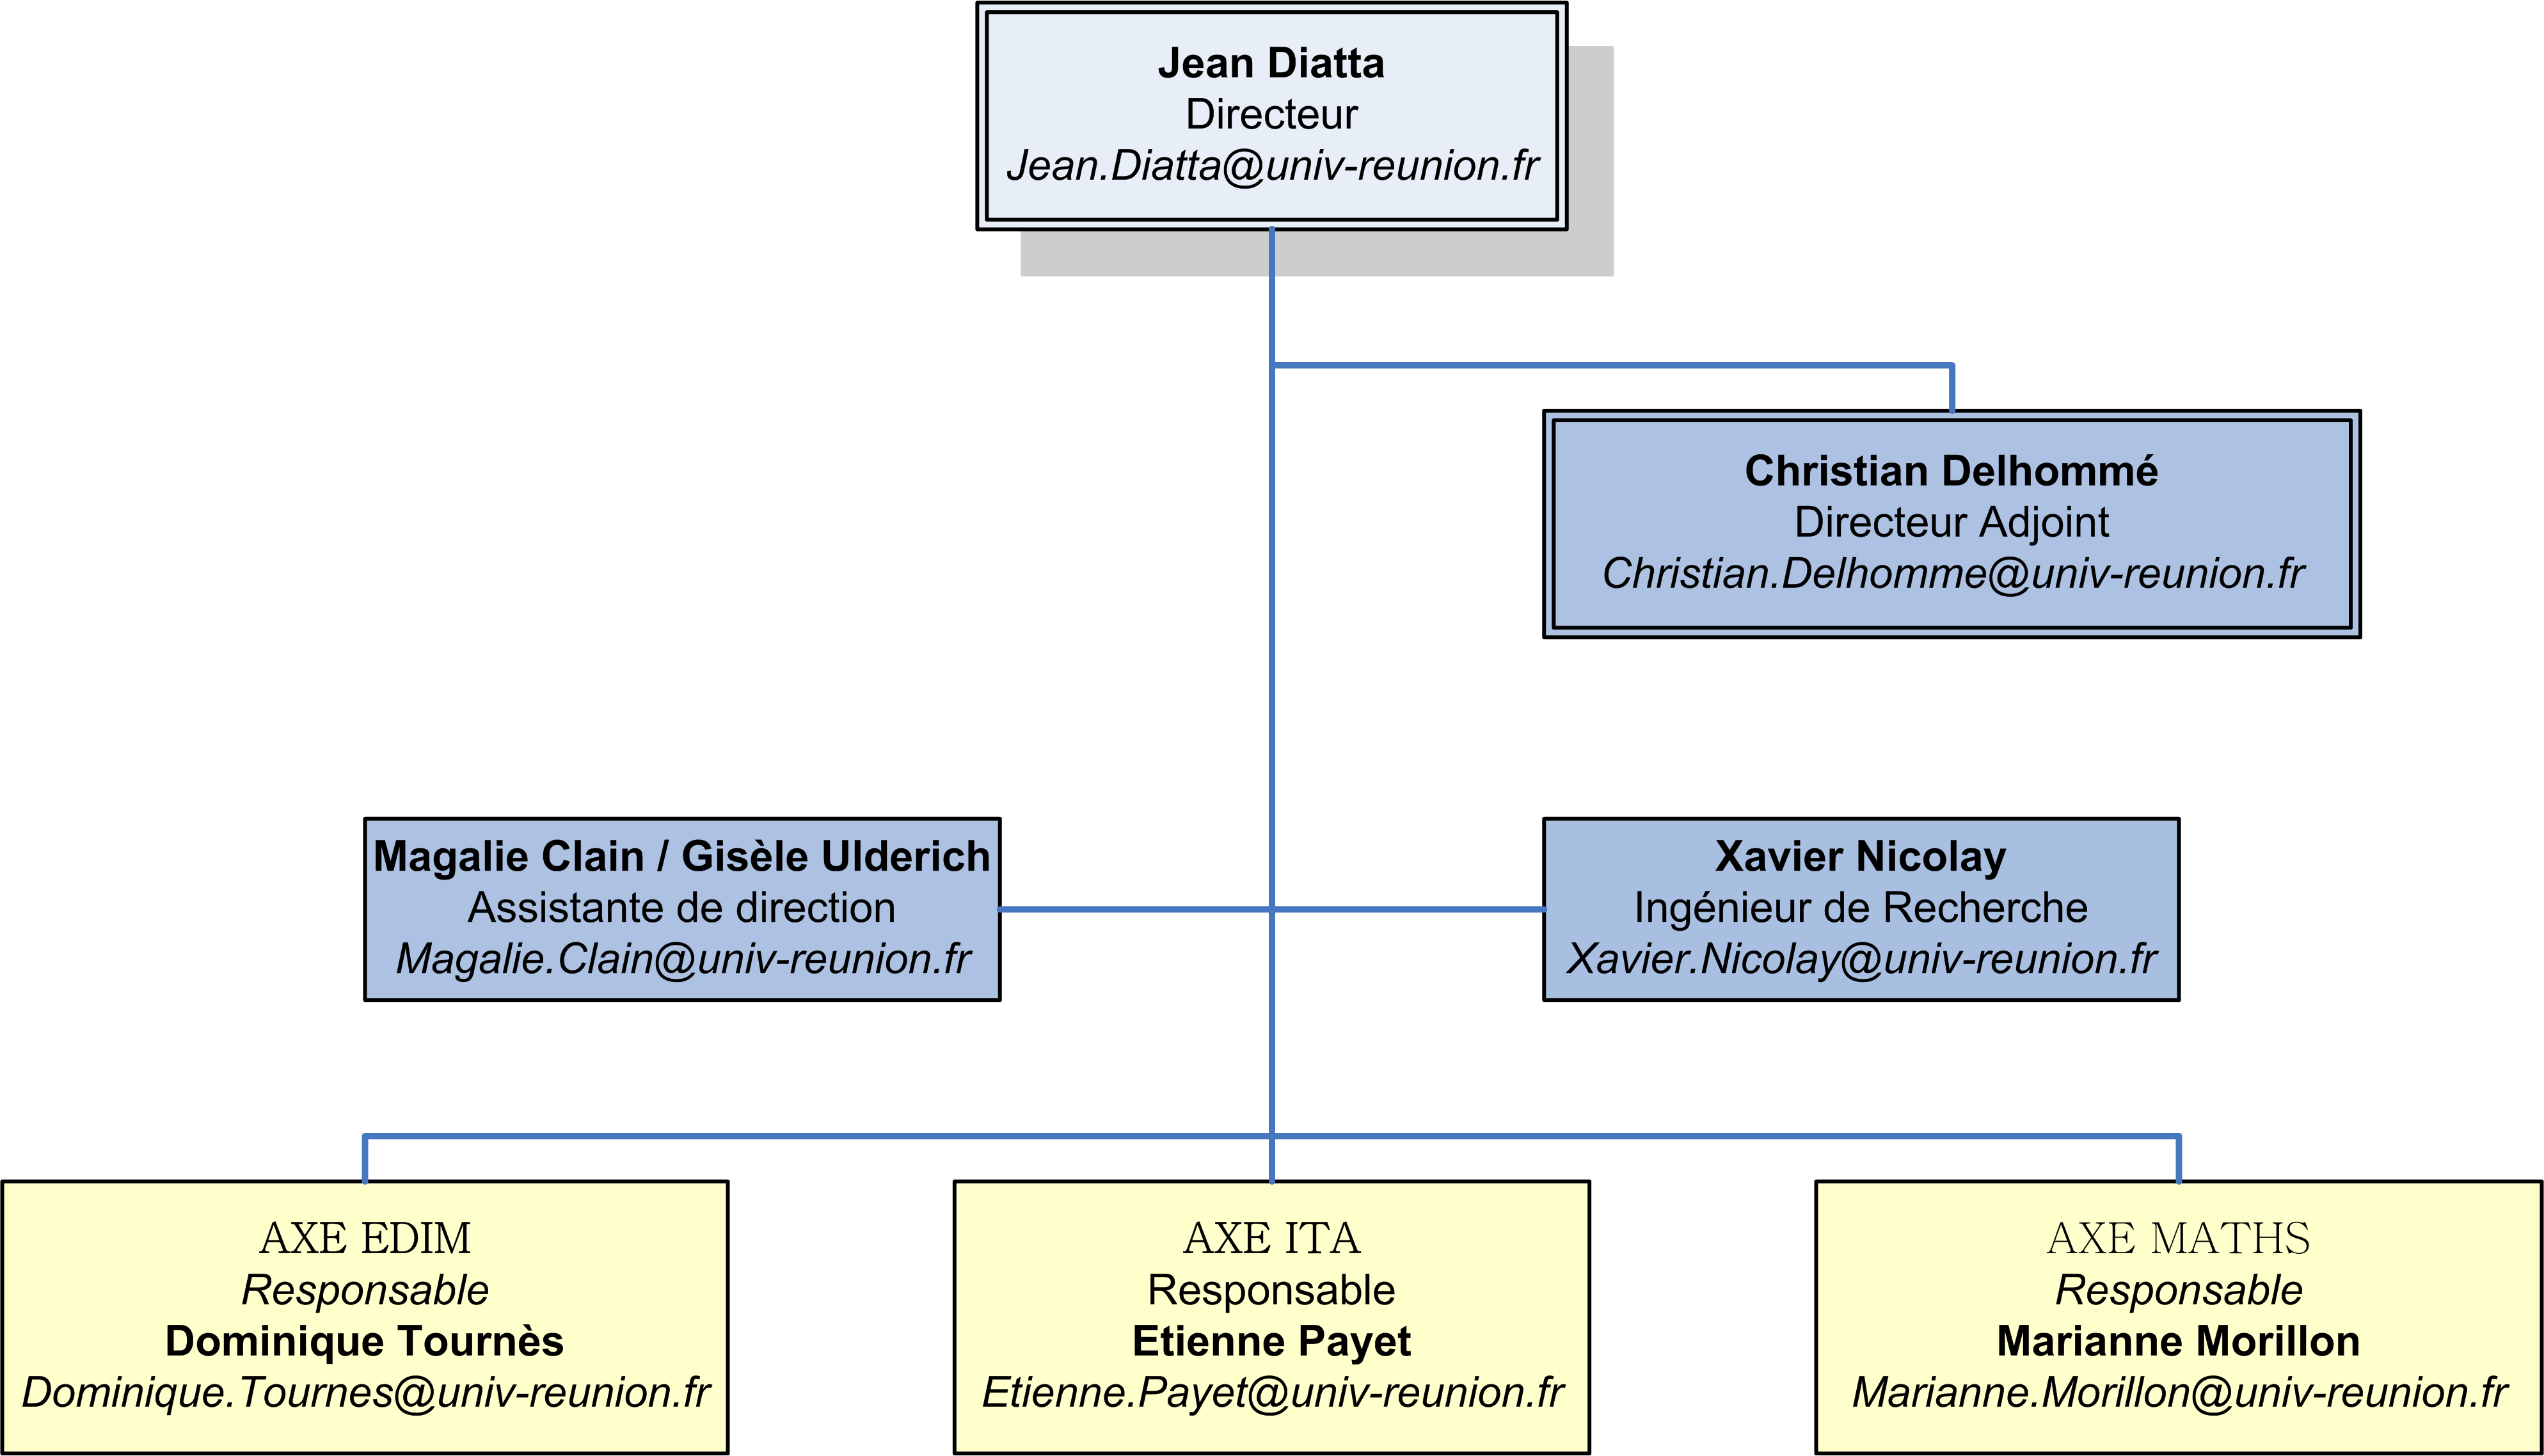
\includegraphics{OrganigrammeLIM-v3.png}
	\end{center}
\end{landscape}

\end{appendices}


 
%                            -=---------------=-
\end{document}
%                            -=---------------=-